\documentclass[11pt, oneside]{article}
\usepackage{geometry}                % See geometry.pdf to learn the layout options. There are lots.
\geometry{letterpaper}                   % ... or a4paper or a5paper or ... 
%\geometry{landscape}                % Activate for for rotated page geometry
%\usepackage[parfill]{parskip}    % Activate to begin paragraphs with an empty line rather than an indent
\usepackage{graphicx}
\usepackage{amsmath}
\usepackage{amsthm}
\usepackage{amssymb}
\usepackage{epstopdf}
%\usepackage{minipage}

\newcommand{\mi}{\operatorname{mi}}


\usepackage{amsthm}
\newcommand{\cV}{\mathcal{V}}

\newtheorem{thm}{Theorem}
\newtheorem{cor}{Corollary}
\newtheorem{lem}{Lemma}
\newtheorem{sch}{Scholium}
%\newtheorem*{conj}{$\Delta^2$ Conjecture}
\newtheorem{defin}{Definition}
\theoremstyle{definition}
\newtheorem{rem}{Remark}
\usepackage[small,nohug,heads=vee]{/Users/Cole/Latex/diagrams}
\newcommand{\Z}{\mathbb{Z}}
\newcommand{\Q}{\mathbb{Q}}
\newcommand{\N}{\mathbb{N}}
\newcommand{\R}{\mathbb{R}}
\newcommand{\C}{\mathbb{C}}
\newcommand{\F}{\mathbb{F}}
\newcommand{\Aut}{\operatorname{Aut}}
\newcommand{\Gal}{\operatorname{Gal}}
\newcommand{\spn}{\operatorname{span}}
\newcommand{\Img}{\operatorname{Im}}
%\newcommand{\ker}{\operatorname{Ker}}


\newtheorem{prop}{Proposition}

\DeclareGraphicsRule{.tif}{png}{.png}{`convert #1 `dirname #1`/`basename #1 .tif`.png}
%\DeclareGraphicsExtensions{.jpeg}

\title{Arrangements with Crossings}
\author{Cole Franks, Andrew Lohr}
%\date{}                                           % Activate to display a given date or no date

\begin{document}
\maketitle
%\section{}
%\subsection{}

\section{Notation}

A finite set of lines $L$ in $\R^2$ partitions the plane into $d$-faces where $d$, signifying dimension, can be zero, one, or two. This notation follows Edelsbrunner \cite{edels}. These faces are points for $d=0$, segments for $d = 1$, and cells for $d=2$. Here cells are what are commonly referred to as faces. This partition is called an \emph{arrangement}, and is denoted $\mathcal{A}(L)$. If no lines are parallel and no three lines intersect in a common point, then the arrangement is called $\emph{simple}$. In this case, if there are $m$ lines then there are exactly ${m \choose 2}$ points of intersection. In this paper all arrangements will be assumed simple.\\

An \emph{arrangement graph} is a graph $G(L)$ defined from $\mathcal{A}(L)$ with vertex set the ${m \choose 2}$ intersections in $\mathcal{A}(L)$ and $v$ and $w$ adjacent in $G(L)$ if and only if $v$ and $w$ are the endpoints of a 1-face, i.e. segment, in $\mathcal{A}(L)$. That is, $v$ and $w$ are on a common line $l$ of $L$, and no other line of $L$ intersects $l$ between $v$ and $w$. Each line intersects $m-1$ other lines, so each line contributes $m-2$ edges to $G(L)$; hence there are $m(m-2)$ total edges in $G(L)$. Note that $G(L)$ is planar, and that the degree of any vertex is either two, three, or four. Lines in the arrangement graph are the paths whose edges correspond to segments of a common line in $\mathcal{A}(L)$. The set of lines in the arrangement graph will be denoted $l(G)$, and for any line $l \in l(G)$, its corresponding line in $\mathcal{A}(L)$ will be denoted $\rho(l)$. Note that arrangement graphs ignore the half-infinite segments.\\



We will study sets of nonintersecting lines in $\R^3$ whose projections to a plane form simple arrangements. We will write elements of $\R^3$ in the standard basis as triples $\vec{r} = (x, y, z)$, and we will assume that we are projecting downward to the $xy$-plane. Let $L$ be a set of nonintersecting lines in $\R^3$. If $l$ is a line in $\R^3$ parameterized by $l(t) = (x(t), y(t), z(t))$, then let $\pi(l)$ denote the line $(x(t), y(t), 0)$ in the $xy$-plane. Suppose additionally that the set $\pi L = \{\pi(l): l \in L\}$ has $\mathcal{A}(L)$ simple. We form a new structure, which we call an \emph{arrangement with crossings}, denoted by $\mathcal{C}(L)$, as follows. 
$\mathcal{C}(L)$ is the pair $(c, \mathcal{A(\pi L)})$, where $c: \pi L \times \pi L \to \{-1, 1\}$ is the \emph{crossing function} defined by $c(\pi(l_1) \pi(l_2)) = 1$ for distinct lines $l_1$ and $l_2$ if and only if $l_1$ passes over $l_2$ in $\R^3$. More precisely, because $\mathcal{A}(\pi L)$ is simple, $\pi(l_1)$ intersects $\pi(l_2)$ at some point $p$. Then $c(\pi(l_1), \pi(l_2)) = 1$ if and only if the $z$-coordinate of the intersection of $l_1$ with the vertical line passing through $p$ is larger than the $z$-coordinate of the intersection of $l_2$ with said line. If $l_1 = l_2$, then $c(\pi(l_1), \pi(l_2))$ is not defined. In any other case, $c(\pi(l_1), \pi(l_2)) = -1$. Note that $c$ is antisymmetric in its arguments. $c$ is called the crossing map, and is only a formal way of describing something familiar: $(c, \mathcal{A}(\pi L))$ is really just a drawing in the plane of lines in $\R^3$ viewed from above, where the crossings are marked as in a knot diagram (see figure \ref{fig:first}). \\

\begin{figure}
\begin{minipage}{\linewidth}
\centering	
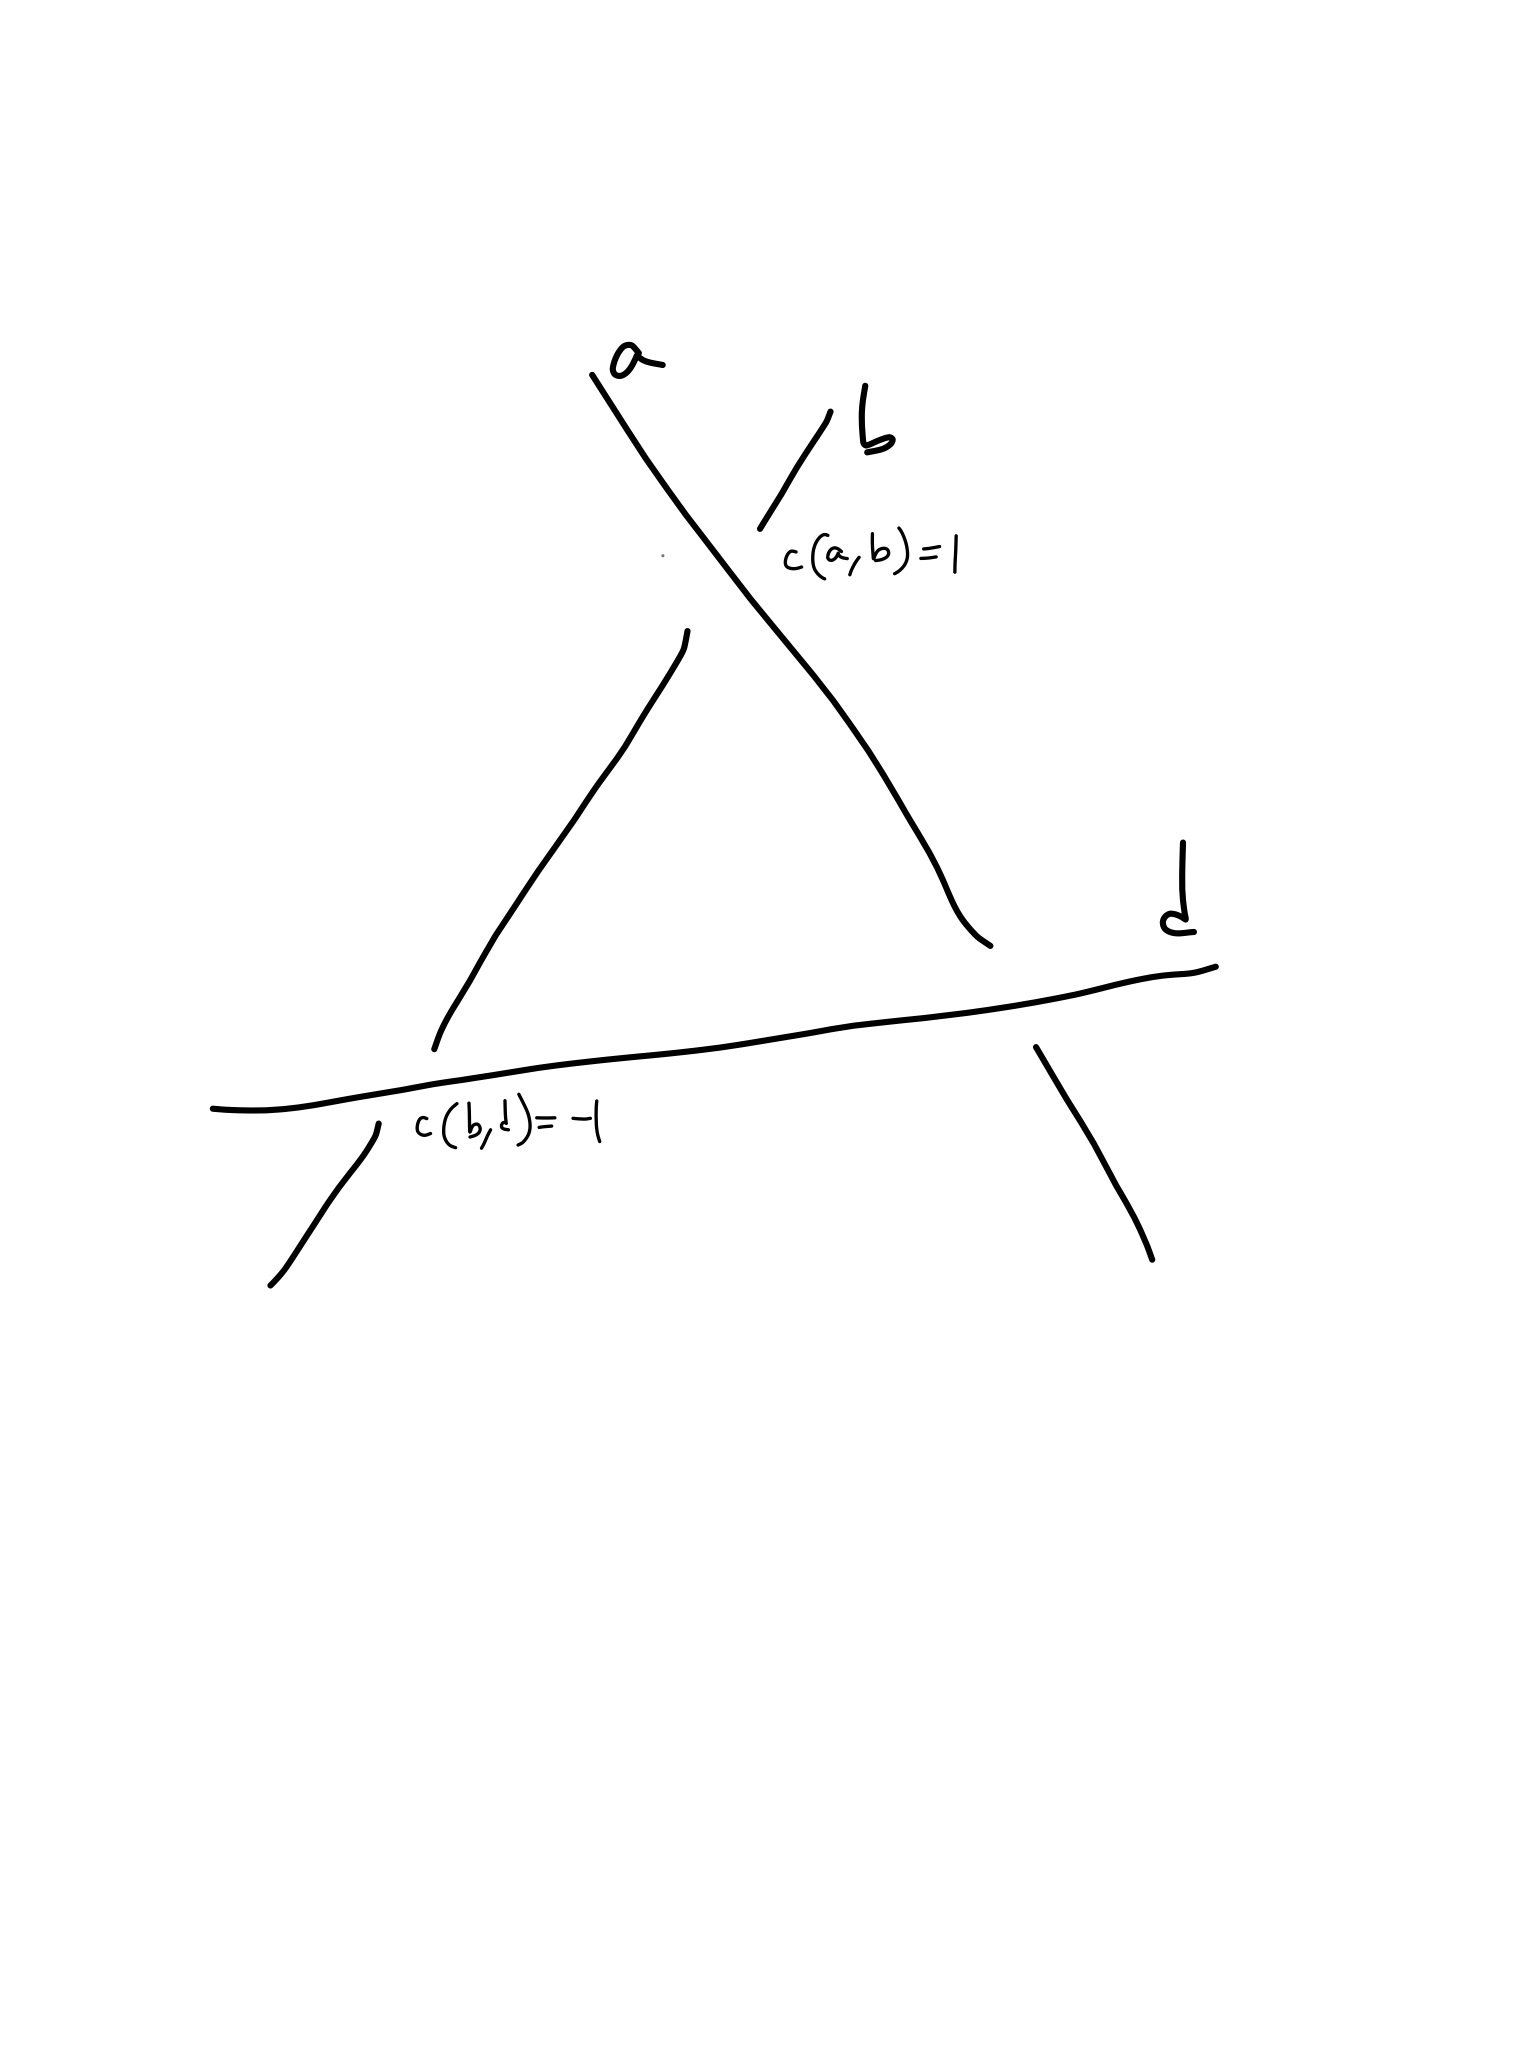
\includegraphics[width=0.9\textwidth]{Arrcross.jpeg}
\caption{Knot diagram interpretation}
\label{fig:first}
\end{minipage}
\end{figure}


The \emph{crossing arrangement graph} is the pair $(c_G, G(\pi L))$, where $c_G: l(G) \times l(G) \to \{-1,1\}$ where $c_G(l_1, l_2) = c(\rho(l_1), \rho(l_2))$. We will refer to $c_G$ as the crossing function for the graph. That is, the crossing map for the crossing arrangement graph is the same crossing map for the arrangement with crossings, only the domain is a set of paths in the graph rather than lines in the plane. 
We will translate the crossing arrangement graph into a directed graph $D(L)$ in the following way. The vertex set of $D(L)$ is the vertex set of $G(\pi L)$, plus one vertex $\mi(e)$ per edge $e$ of $G(\pi L)$. The graph will be bipartite and directed. The only edges will be of the form $\mi(e)v$ or $v \mi(e)$ for $e \in E(G(\pi L))$ and $v \in e$. Let $l_1$ and $l_2$ in $l(G)$ be lines such that $e$ belongs to $l_1$ and $v = l_1 \cap l_2$. 
These lines are uniquely defined, because each point is the intersection of exactly two lines and each edge is in exactly one line. Then $\mi(e)v$ is an edge in $D(L)$ if and only if $c_G(l_1, l_2) = 1$, and $v \mi(e)$ is an edge in $D(L)$ if and only if $c_G(l_1, l_2) = -1$. See figure \ref{fig:second}. $D(L)$ has $|E(G(L))| +  |V(G(L))| = m(m-2) + { m \choose 2}$ vertices and $2m(m-2)$ edges. \\

\begin{figure}
\begin{minipage}{\linewidth}
\centering
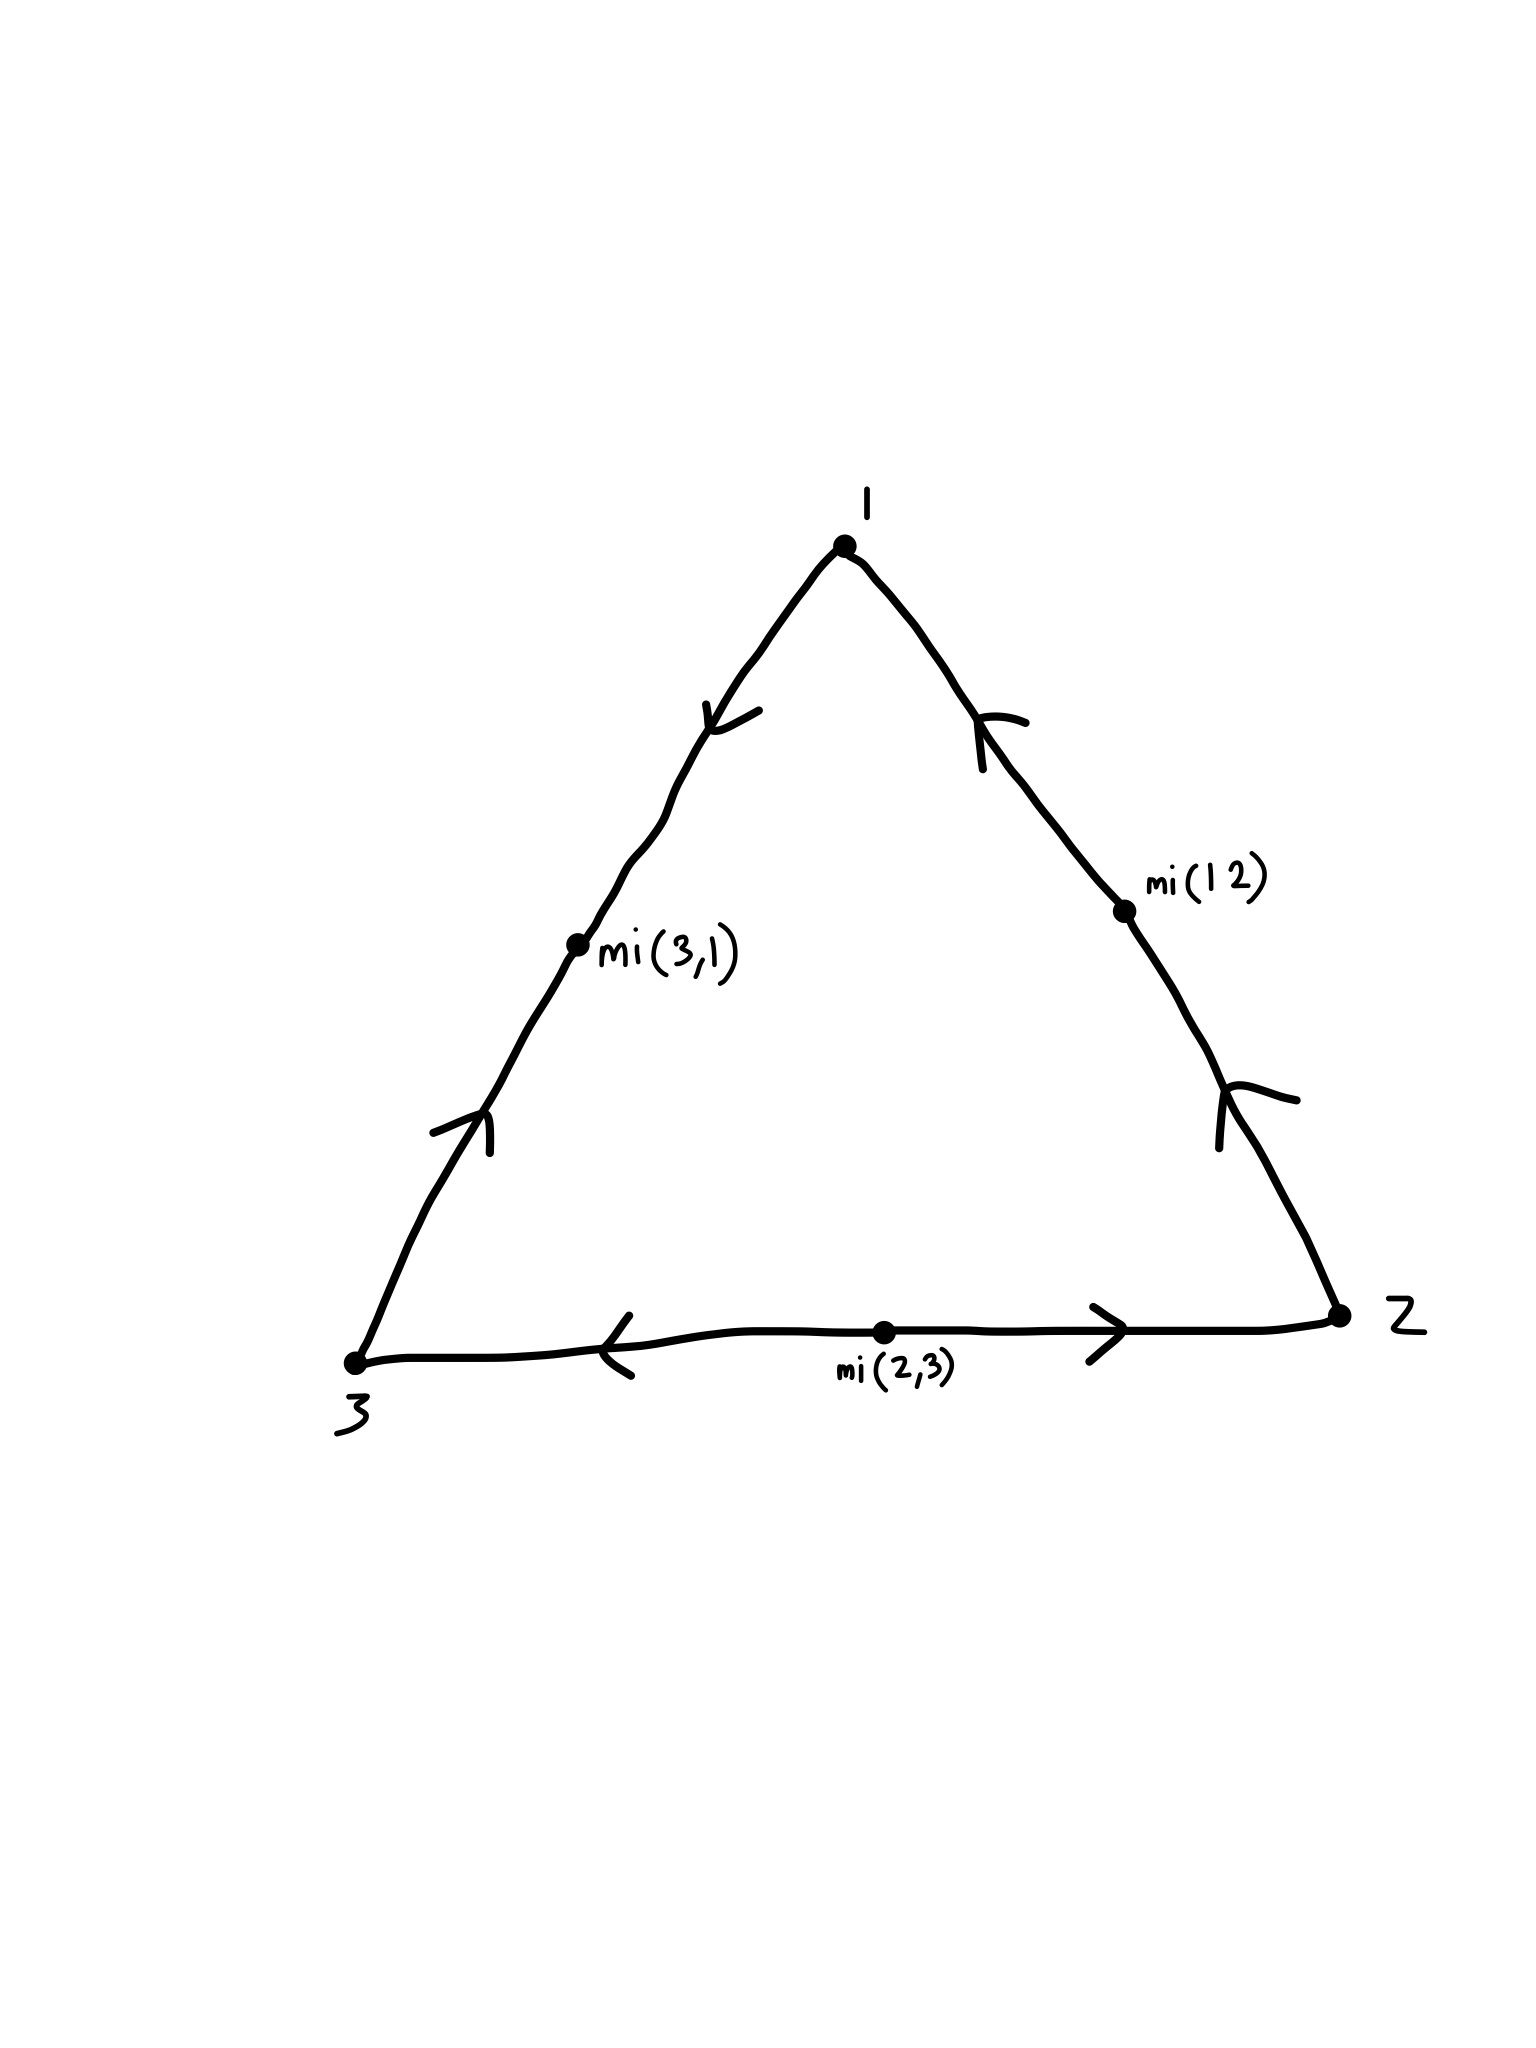
\includegraphics[width=0.9\textwidth]{Digraph.jpeg}
\caption{Crossing arrangement graph}
\label{fig:second}
\end{minipage}
\end{figure}





Throughout this paper, if $G$ is a graph, $V(G)$ is the vertex set of $G$ and $E(G)$ is the edge set.

\section{Geometric to Combinatorial}
The goal of this section is to show that $D(L)$ and $D(L')$ isomorphic as graphs if and only if $\mathcal{C}(L) = (c, \mathcal{A}(L))$ and $\mathcal{C}(L') = (c', \mathcal{A}(L'))$ are isomorphic in a certain sense.\\

 First, we say that two arrangements $\mathcal{A }(L)$ and $\mathcal{A} (L')$ are isomorphic if there is a homeomorphism $h$ of $\R^2$ carrying $\mathcal{A }(L)$ to $\mathcal{A} (L')$ in the sense that for each $d$-face $X$ of $\mathcal{A}(L)$, we have $h|_X: X \to Y$ is a homeomorphism of $X$ and $Y$ where $Y$ is a $d$-face of $\mathcal{A}(L')$. 
 This means that points map to points, segments map to segments homeomorphically, and cells map to cells homeomorphically. In this case we refer to $h$ as an isomorphism of arrangements, and write $\mathcal{A }(L) \cong \mathcal{A} (L')$. \\




We say that $\mathcal{C}(L) = (c, \mathcal{A}(L))$ and $\mathcal{C}(L')  = (c', \mathcal{A}(L'))$ are isomorphic if there is an isomorphism of arrangements $h:\mathcal{A }(\pi L) \to \mathcal{A} (\pi L')$ such that for any two lines $l_1$ and $l_2$ in $\pi L$, $c(l_1, l_2) = c'(h(l_1), h(l_2))$, and the lefthand side is defined if and only if the right hand side is. 
Similarly, their crossing arrangement graphs are isomorphic if there exists a graph isomorphism $G( \pi L) \to G( \pi L')$ that preserves the crossing function $c_G$. This definition only makes sense if $h(l)$ is a line in $\mathcal{A}(\pi L')$ for any $l \in \pi L$, which we will show is the case. 
 \begin{lem}
Let $L, L'$ be finite sets of lines in the plane. If $h: \mathcal{A}(L) \to \mathcal{A}(L')$ is an isomorphism of (simple) arrangements, then any line in $L$ is mapped homeomorphically by $h$ to a line of $L'$. 
 \end{lem}
\begin{proof}
Let $e_0$ be one of the infinite segments of $l$. Then $h(e_0)$ is another infinite segment, say $f_0$, for this is the only type of face that is homeomorphic to $e_0$. Let $v_0$ be the endpoint of $e_0$. 
Consider the segments $e_1, e_2, e_3$ that border $e_0$ at $v$ in clockwise order starting at $e_0$. Observe that $e_2 \subset l$. Let $l'$ be the line to which $f_0$ belongs and let $w_0$ be the endpoint of $f_0$. Again, we consider the segments $f_1, f_2, f_3$ that border $f_0$ at $w_0$ in clockwise order starting at $f_0$. $f_2 \subset l'$. We claim that $h(e_2) = f_2$. 
Because $h$ is a homeomorphism, we know that $h(e_2)$ is a segment bordering $f_0$ at $w_0$. Suppose $h(e_2) = f_1$. Then we must have $\{h(e_1),h(e_3)\} = \{f_2, f_3\}$. \\

 $l$ cuts the plane into two disjoint open half-planes, $P_1$ containing $e_1$ and $P_3$ containing $e_3$. $h(l)$ is an unbounded polygonal curve that separates the plane into two disjoint regions $R_1$ and $R_3$. 
 $h(l)$ is unbounded because the half infinite segments belonging to $l$ must map to half infinite segments in $\mathcal{A}(L')$, and it separates the plane into two regions by the Jordan curve theorem applied to the stereographic projection of the plane. 
 Because $h$ is a homeomorphism, we have $h(P_i) = R_i$ without loss of generality. Now note that both $f_2$ and $f_3$ are contained together in one of $h(P_1)$ or $h(P_3)$; however, $h(e_1) =f_1\subset h(P_1)$ and $h(e_3) = f_3 \subset h(P_3)$. This is impossible because $h(P_3) \cap h(P_1) = \emptyset$. \\
 
 Identical reasoning can be applied to the case $h(e_2) = f_3$, so we conclude $h(e_2) = f_2$. This reasoning can be applied inductively to see that the $i^{th}$ segment of $l$ counting away from $e_0$, must map to the $i^{th}$ segment of $l'$ counting away from $f_0$. Hence, $h(l) = l'$. 
 \end{proof}
 
\begin{lem}
Two simple arrangements $\mathcal{A}(L)$ and $\mathcal{A}(L')$ are isomorphic if and only if their arrangement graphs $G(L)$ and $G(L')$ are isomorphic as graphs. In particular, 
\end{lem}

\begin{proof}
Suppose $\phi: G(L) \to G(L')$ is an isomorphism. Let $\nu:G(L) \to \mathcal{A}(L)$ be the natural map sending the edges and vertices of $G(L)$ into the corresponding points and segments of $\mathcal{A}(L)$, which is an embedding of $G(L)$ as a plane graph. 
Note that the vertices of degree at most three in $G(L)$ are exactly those on the unbounded face in this embedding (these are the endpoints of the unbounded segments).  $\nu': G(L') \to \mathcal{A}(L')$ is an embedding of $G(L')$ with the same property. 
Then $\nu' \circ \phi$ is an embedding of $G(L)$, the image of which is identical to the embedding of $G(L')$. Following \cite{bose}, we define a new graph $G(L)^*$ that is an identical copy of $G(L)$ plus a new vertex, $x$, that is attached to all vertices of degree at most three. 
Because both embeddings, $\nu$ and $\nu'\circ\phi$, of $G(L)$ have all vertices of degree two and three on the unbounded face, there exist embeddings $\mu$ and $\mu'$ of $G(L)^*$ extending $\nu$ and $\nu' \circ \phi$, respectively. 
Namely, in both embeddings, $x$ goes in the unbounded face and connects to all vertices on the unbounded face. From \cite{bose}, $G(L)^*$ is three-connected. 
By a theorem originally due to Whitney \cite{diestel}, all embeddings of $G(L)^*$ with $x$ on the unbounded face are equivalent, meaning there is a homeomorphism $h:\mu(G(L)^*) \to \mu'(G(L)^*)$ such that $h$ extends the set map $\mu' \circ \mu^{-1}$ on the vertices and edges. As $\mu' \circ \mu^{-1}$ maps $x$ to $x$, we must have $h: \nu(G(L)) \to \nu' \circ \phi((G(L))$. 
Furthermore, $h$ must also extend the set map $\nu' \circ \phi \circ \nu^{-1}$.

If $h:\mathcal{A}(L) \to \mathcal{A}(L')$ is an isomorphism of arrangements, then one can easily see that the map induced by $h$ on the vertices of $G(L)$ provides an isomorphism with $G(L')$. \end{proof}
 
 \begin{lem}\label{cgraphtoarr}
Two arrangements with crossings $\mathcal{C}(L)$ and $\mathcal{C}(L')$ are isomorphic if their crossing arrangement graphs $(c_G, G(\pi L))$ and $(c'_G, G(\pi L'))$ are isomorphic.
\end{lem}

\begin{proof}
Let $\phi:(c_G, G(\pi L)) \to (c_G, G(\pi L')$ be an isomorphism. $\phi$ is also an isomorphism of graphs $G( \pi L) \to G( \pi L')$. 
From the previous lemma we know $\mathcal{A}(L)$ and $\mathcal{A}(L')$ are isomorphic under an isomorphism or arrangements $\psi$ extending $\nu' \circ \phi \circ \nu^{-1}$ on the vertices. 
We have defined for lines $l_1, l_2 \subset G( \pi L)$, $c_G(l_1, l_2) = c(\nu (l_1), \nu (l_2))$; likewise for $c'$. Then $$c_G'(\phi (l_1), \phi (l_2)) = c'(\nu' \phi (l_1), \nu' \phi (l_2)) = c' (\psi \circ \nu (l_1), \psi \circ \nu (l_2)).$$ 
But $\phi$ is an isomorphism of crossing arrangement graphs, so 
$$c_G'(\phi (l_1), \phi (l_2))= c_G(l_1, l_2) = c(\nu (l_1), \nu (l_2)).$$
In particular, $c' (\psi \circ \nu (l_1), \psi \circ \nu (l_2))= c(\nu (l_1), \nu (l_2))$. As $\nu$ is a bijection, we see that $\psi$ is an isomorphism of arrangements with crossings. \end{proof}

\begin{lem}\label{dirtograph}
If $|L|=m > 3$, $D(L) \cong D(L') \implies (c_G, G(\pi L))\cong (c'_G, G(\pi L'))$.
\end{lem}
\begin{proof}
Let $\phi: D(L) \to D(L')$ be an isomorphism of directed graphs. First we claim that the set $M_L = \{ \mi(e): e \in G( \pi L)\} \subset V(D(L))$ is mapped to the corresponding set $M_{L'} \subset V(D(L'))$ by $\phi$. 
Note that the undirected distance $d(\mi(e), v)$ for $\mi(e) \in M_L$ and $v \in V(D(L) \setminus M_L$ is always odd, and $d(\mi(e_1), \mi(e_2))$ is always even. 
This is because the $\mi(e)$ are midpoints inserted into edges of the graph $G(L)$. The same distance condition holds for $M_{L'}$ and $V(D(L')) \setminus M_{L'}$. Hence, we must have either $\phi M_{L} = M_{L'}$ or $\phi M_{L} = V(D(L')) \setminus M_{L'}$, because isomorphisms preserve distance.
 Let $m' = |L'|$. Recall that $|V(D(L'))| = m'(m'-2) + {m' \choose 2}$, which is monotone increasing for $m' > 2$, so we must have $m' = m$ because $|V(D(L') = V(D(L))| = m(m-2) + {m \choose 2}$. 
 Then $|M_L| = |M_{L'}|= m(m-2)$, and $V(D(L')) \setminus M_{L'} = {m \choose 2}$. According to Maple, $m(m-2) > { m \choose 2}$ for $m > 3$, so we must have $\phi M_{L} = M_{L'}$ as desired. 
 Hence we also have $\phi  V(D(L)) \setminus M_{L} = V(D(L')) \setminus M_{L'}$, which indicates that the subset of $V(D(L))$ corresponding to vertices in $V(G(L))$ are mapped to those corresponding to vertices in $V(G(\pi L'))$. \\

Viewing $V(G( \pi L)), V(G( \pi L'))$ as a subsets of $V(D(L))$ and $V(D(L'))$, respectively, we claim that $\psi = \phi|_{V(G(\pi L))}:V(G( \pi L)) \to V(G( \pi L'))$ is an isomorphism. 
We have just shown that the codomain of $\psi$ is within (and hence all of, by injectivity) $V(G(\pi L'))$, so it remains only to show that it is an isomorphism of arrangement graphs with crossings. First, it is a graph isomorphism. A fortiori, $\phi$ is an undirected graph isomorphism $D(L) \to D(L')$. If $vw \in E(G( \pi L))$, then $v\mi(vw)w$ is an undirected $2$-path in $D(L)$. 
$\phi(v) \phi(\mi (vw)) \phi (w)$ remains an undirected $2$-path in $D(L')$. As we showed in the previous paragraph, $\phi(v) = \psi(v)$ and $\phi(w)= \psi(w)$ are in $V(G( \pi L'))$. 
In $D(L')$ they are only connected to vertices of the form $\mi (e)$ for $e \in E(G(\pi L))$, and each such $\mi(e)$ has only two neighbors. As $\psi(v)$ and $\psi(w)$ have a common neighbor in $D(L')$, we can deduce that it is $\mi(\psi(v)\psi(w))$, and hence that $\psi(v)\psi(w) \in E(G(\pi L'))$. 
In particular, $\phi(\mi(vw)) = \mi(\psi(v) \psi(w)$. The same argument applied to $\phi^{-1}$ shows if $vw \notin E(G(\pi L))$, then $\psi(v)\psi(w) \notin E(G( \pi L'))$.\\

Now we show that $c'_G(\psi(l_1), \psi(l_2) = c_G(l_1, l_2)$ for distinct lines $l_1, l_2 \subset G(\pi L)$. Suppose $l_1$ and $l_2$ cross at $v$, and that $w_1$ and $w_2$ are vertices on $l_1$ and $l_2$, respectively, that are adjacent to $v$. Assume $c_G(l_1, l_2) =1$. 
Then we have directed edges $\mi(vw_1)v$ and $ v \mi(vw_2) \in E(D(L))$. As $\phi$ is an isomorphism of directed graphs, $\phi(\mi(vw_1)\psi(v))\psi(v) = \mi (\psi(v)\psi(w_1))\psi(v)$ and $\psi(v)\mi (\psi(v)\psi(w_2))$ are directed edges of $D(L')$. 
We know $\psi(l_i)$ is the line containing $\psi(v)$ and $\psi(w_i)$, for $i=1,2$. By definition of $D(L')$, we have $c'_G(\psi(l_1), \psi(l_2)) = 1$. The $-1$ case follows by antisymmetry (we can swap $l_1$ and $l_2$). Hence, $\psi$ is an isomorphism of arrangement graphs with crossings. 
\end{proof}

\begin{thm} For $L, L'$ finite sets of nonintersecting lines in $\R^3$ with $|L| > 3$, the following are equivalent:
\begin{enumerate}
\item $D(L) \cong D(L')$. \label{directeds}
\item $(c_G, G(\pi L))\cong (c'_G, G(\pi L'))$. \label{crossgraph}
\item $\mathcal{C}(L) \cong \mathcal{C}(L')$. \label{crossarr}
\end{enumerate}
\end{thm}

\begin{proof}
A moments' thought shows that $\ref{crossarr} \implies \ref{directeds}$.  Lemma $\ref{dirtograph}$ gives $\ref{directeds} \implies \ref{crossgraph}$. Lemma $\ref{cgraphtoarr}$ gives $\ref{crossgraph} \implies \ref{crossarr}$. \end{proof}
 
 
 %$k$ also determines an open half plane containing $e_2$ which we will call $P_2$. Since $l$ and $k$ cross, $P_1 \cap P_2$ is a region homeomorphic to a plane (a nonempty infinite sector), and $P_1 \Delta P_2$ the union of two sectors with endpoints at the origin. $h(l)$ is also an unbounded polygonal curve that separates the plane into two regions, one of which is $h(P_1)$. $h(l)$ is unbounded because the half infinite segments belonging to $l$ must map to half infinite segments in $\mathcal{A}(L')$, and it separates the plane into two regions by the Jordan curve theorem applied to the stereographic projection of the plane. Similarly, $h(k)$ is an unbounded polygonal curve that separates the plane into two regions, one of which is $h(P_2)$. Let $B$ be a small ball around $w_0$, so small that $B$ only intersects the cells and segments that meet $w_0$, and further small enough that $h^{-1}(B)$ only intersects the cells and segments that meet $v_0$. Then $h(P_1) \cap B$ and $h(P_2) \cap B$ are homeomorphic to sectors. $h^{-1}(h(P_1) \cap h(P_2) \cap B) = P_1 \cap P_2$, and $h^{-1}((h(P_1) \Delta h(P_2)) \cap B) = P_1 \Delta P_2$. 



\bibliographystyle{plain}
\bibliography{cheez1}


 
\end{document}  
